\documentclass[aspectratio=169]{beamer}
%% deck-source-version: 1
% ---- ツール管理プリアンブル(将来は deck init / deck format が生成・所有する)----
\usetheme{default}
\setbeamertemplate{navigation symbols}{}
\usepackage{graphicx}
\usepackage{amsmath}
\usepackage{amssymb}
\usepackage{booktabs}
\usepackage{hyperref}
% ---- ツール管理ここまで ----

%% macros:begin
\newcommand{\code}[1]{\texttt{#1}}
\def\emphpair(#1,#2){\textbf{#1}/\textit{#2}}
%% macros:end

%% preamble-extra:begin
% サブセット外パッケージはこの自由領域に書く(ツールは素通しする)
\usepackage{tikz}
\usepackage[normalem]{ulem}
%% preamble-extra:end

\title{Kitchen Sink}
\subtitle{Golden sample: deliberately outside the subset}
\author{Beamer Editor Team}
\date{2026-07-10}

\begin{document}

\begin{frame}
  \titlepage
\end{frame}

\begin{frame}{Still a normal frame}
  \begin{itemize}
    \item Subset content coexists with raw blocks in the same deck.
    \item Everything below this frame degrades gracefully.
  \end{itemize}
\end{frame}

\begin{frame}{A TikZ picture}
  % 未知環境 → ブロック生ブロック(プレビューは部分コンパイル画像)
  \begin{center}
    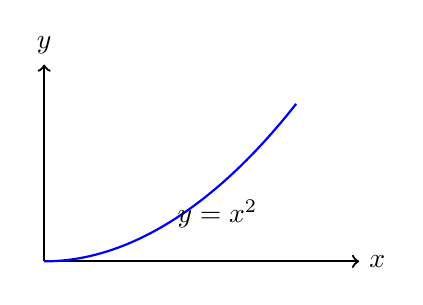
\begin{tikzpicture}
      \draw[thick,->] (0,0) -- (4,0) node[right] {$x$};
      \draw[thick,->] (0,0) -- (0,2.5) node[above] {$y$};
      \draw[blue,thick] (0,0) parabola (3.2,2.0);
      \node at (2.2,0.6) {$y = x^{2}$};
    \end{tikzpicture}
  \end{center}
\end{frame}

\begin{frame}{Overlay commands outside the subset}
  % \only / \uncover は v1 対象外 → インライン生ブロック
  \only<1>{This line uses only, visible on step one.}
  \uncover<2->{This line uses uncover, from step two onward.}
\end{frame}

\begin{frame}[fragile]{Verbatim requires fragile}
  \begin{verbatim}
deck lint slides/main.tex --json
deck check slides/main.tex
  \end{verbatim}
\end{frame}

\begin{frame}{A table beyond the subset}
  % 縦罫線と multicolumn は対象外 → 環境ごと生ブロック
  \begin{center}
    \begin{tabular}{|l|c|}
      \hline
      \multicolumn{2}{|c|}{Header spanning both columns} \\
      \hline
      alpha & 1 \\
      beta & 2 \\
      \hline
    \end{tabular}
  \end{center}
\end{frame}

\begin{frame}{Macro calls that fall back}
  A delimited macro call \emphpair(alpha,beta) becomes a raw block, as do
  \sout{struck text}, \fbox{a framed box}, and this footnote.\footnote{Footnotes are outside the subset too.}
\end{frame}

\begin{frame}{Math beyond the subset}
  % gather* はサブセット外の数式環境 → 生ブロック
  \begin{gather*}
    a = b + c \\
    d = e - f
  \end{gather*}
\end{frame}

\begin{frame}[shrink=5]{A frame the parser gives up on}
  % 未知のフレームオプション → フレーム全体が生フレーム(一覧・並べ替えのみ可能)
  This whole frame becomes a raw frame because of the unknown option, but it
  still compiles and still shows up in the slide list.
\end{frame}

\begin{frame}{Summary}
  \begin{itemize}
    \item Out-of-subset syntax never breaks the deck.
    \item It only degrades the preview and the GUI, never the PDF.
  \end{itemize}
\end{frame}

\end{document}
